\documentclass{beamer}
\usepackage{hyperref} %ctex,
\usepackage[english]{babel}
\usepackage[T1]{fontenc}

% other packages
\usepackage{latexsym,amsmath,xcolor,multicol,booktabs,calligra}
\usepackage{graphicx,pstricks,listings,stackengine}

\author{Olle Rehnfeldt, Jakob Hutter}
\title{ADAM}
\subtitle{Adaptive Movement Estimation Algorithm}
\institute{Data Science and Society}
\date{\today}

% defs
\def\cmd#1{\texttt{\color{red}\footnotesize $\backslash$#1}}
\def\env#1{\texttt{\color{blue}\footnotesize #1}}
\definecolor{deepblue}{rgb}{0,0,0.5}
\definecolor{deepred}{rgb}{0.6,0,0}
\definecolor{deepgreen}{rgb}{0,0.5,0}
\definecolor{halfgray}{gray}{0.55}

\lstset{
    basicstyle=\ttfamily\small,
    keywordstyle=\bfseries\color{deepblue},
    emphstyle=\ttfamily\color{deepred},    % Custom highlighting style
    stringstyle=\color{deepgreen},
    numbers=left,
    numberstyle=\small\color{halfgray},
    rulesepcolor=\color{red!20!green!20!blue!20},
    frame=shadowbox,
}

\newcommand\myheading[1]{%
  \par\bigskip
  {\Large\bfseries#1}\par\smallskip}


\begin{document}

\begin{frame}
    \titlepage
\end{frame}


\begin{frame}
    \myheading{Gradient Descent}
    What is gradient Descent
\end{frame}


\begin{frame}
    \myheading{Stochastic Gradient Descent}
    What is SGD
\end{frame}

\begin{frame}
    \myheading{What is ADAM doing?}
\end{frame}
\begin{frame}
    \myheading{Improving Stochastic Gradient Descent for Training Neural Networks.}
\end{frame}


\begin{frame}
    \myheading{Momentum Method\\First Moment Vector}
    Step direction is dependent on current and past gradients.
    $$Next Step = constant \cdot last step + (1-constant) \cdot Gradient$$
    
    \begin{figure}[h]
        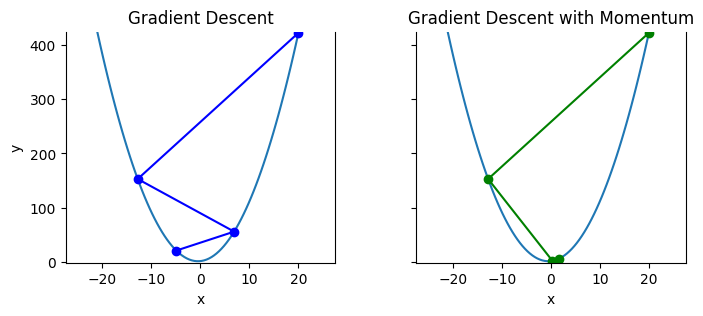
\includegraphics[width=8cm]{report/figures/GD_momentum.png}
    \end{figure}
\end{frame}


\begin{frame}
    \myheading{Adaptive Learning Rate\\Second Moment Vector}
    Step Length is dependent on magnitude of the gradient
    $$NextStepSize = \frac{LearningRate}{Gradient^2} $$
    
    \begin{figure}[h]
        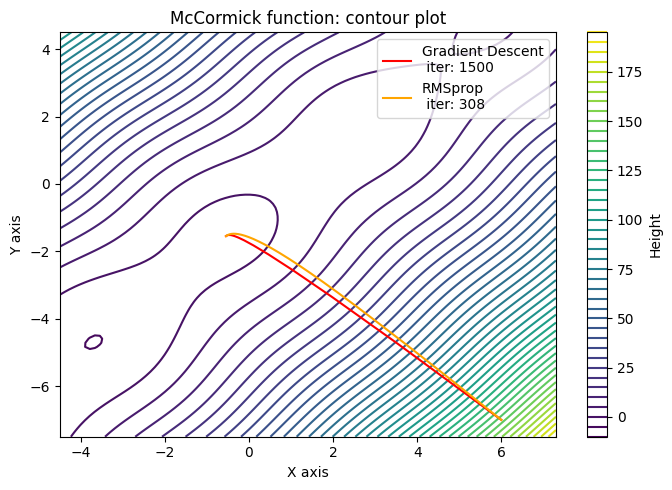
\includegraphics[width=8cm]{report/figures/GD_rmsprop.png}
    \end{figure}
\end{frame}


\begin{frame}
    \myheading{Bias correction}
    Both methods are initialized as zeros.
    
    \begin{figure}[h]
        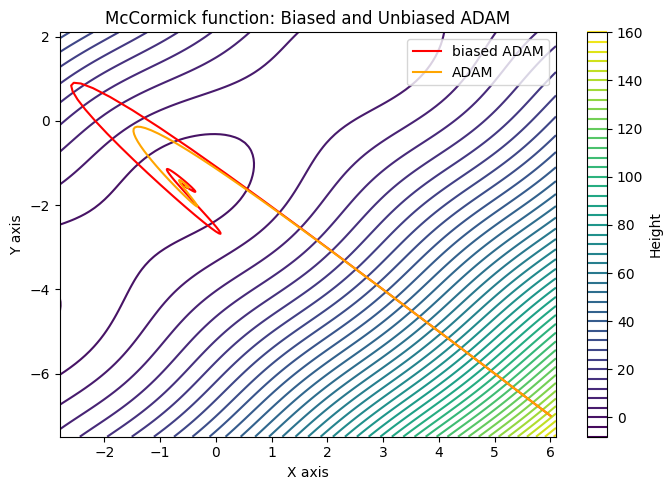
\includegraphics[width=8cm]{report/figures/ADAM_bias.png}
    \end{figure}
\end{frame}



\begin{frame}
    \myheading{ADAM}
    Stochastic Gradient Descent with
    \begin{enumerate}
        \item Momentum Method
        \item Adaptive Learning Rate
        \item Bias correction
    \end{enumerate}
    
    \begin{figure}[h]
        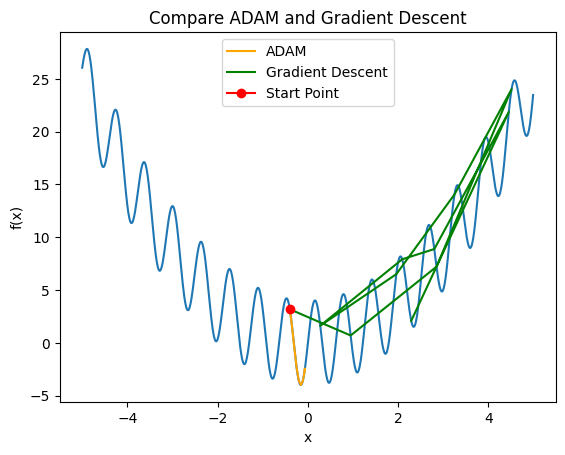
\includegraphics[width=8cm]{report/figures/adam_vs_gradientdescent.png}
    \end{figure}
\end{frame}

\begin{frame}
    \myheading{The Algorithm}
    \begin{enumerate}
        \item Initialize Parameters
        Neural Network Weights, Constants, etc.
        \item Initialize First and Second Moment Vector as vectors of 0
        \item Calculate the Gradient of the loss function with the current batch
        \item Calculate the First Moment vector, remove bias
        \item Calculate the Second Moment vector, remove bias
        \item Calculate the adapted new set of parameters
        \item If the parameters converge stop, otherwise go back to step 3. With next batch
    \end{enumerate}
\end{frame}




\begin{frame}
    \myheading{Advantages of ADAM}
\end{frame}

\begin{frame}
    \myheading{Test Set MNIST-Fashion}
    \begin{enumerate}
        \item 70000, 28x28 images, pixel darkness value ranging 0-255 (normalized before prediction)
        \item 10 different classes of fashion items: T-shirt/top, Trouser, Pullover, Dress, Coat,
               Sandal, Shirt, Sneaker, Bag, Ankle boot.
        \item Advantageous to the regular MNIST data set. 
    \end{enumerate}
\end{frame}

\begin{frame}
     \begin{figure}[h]
        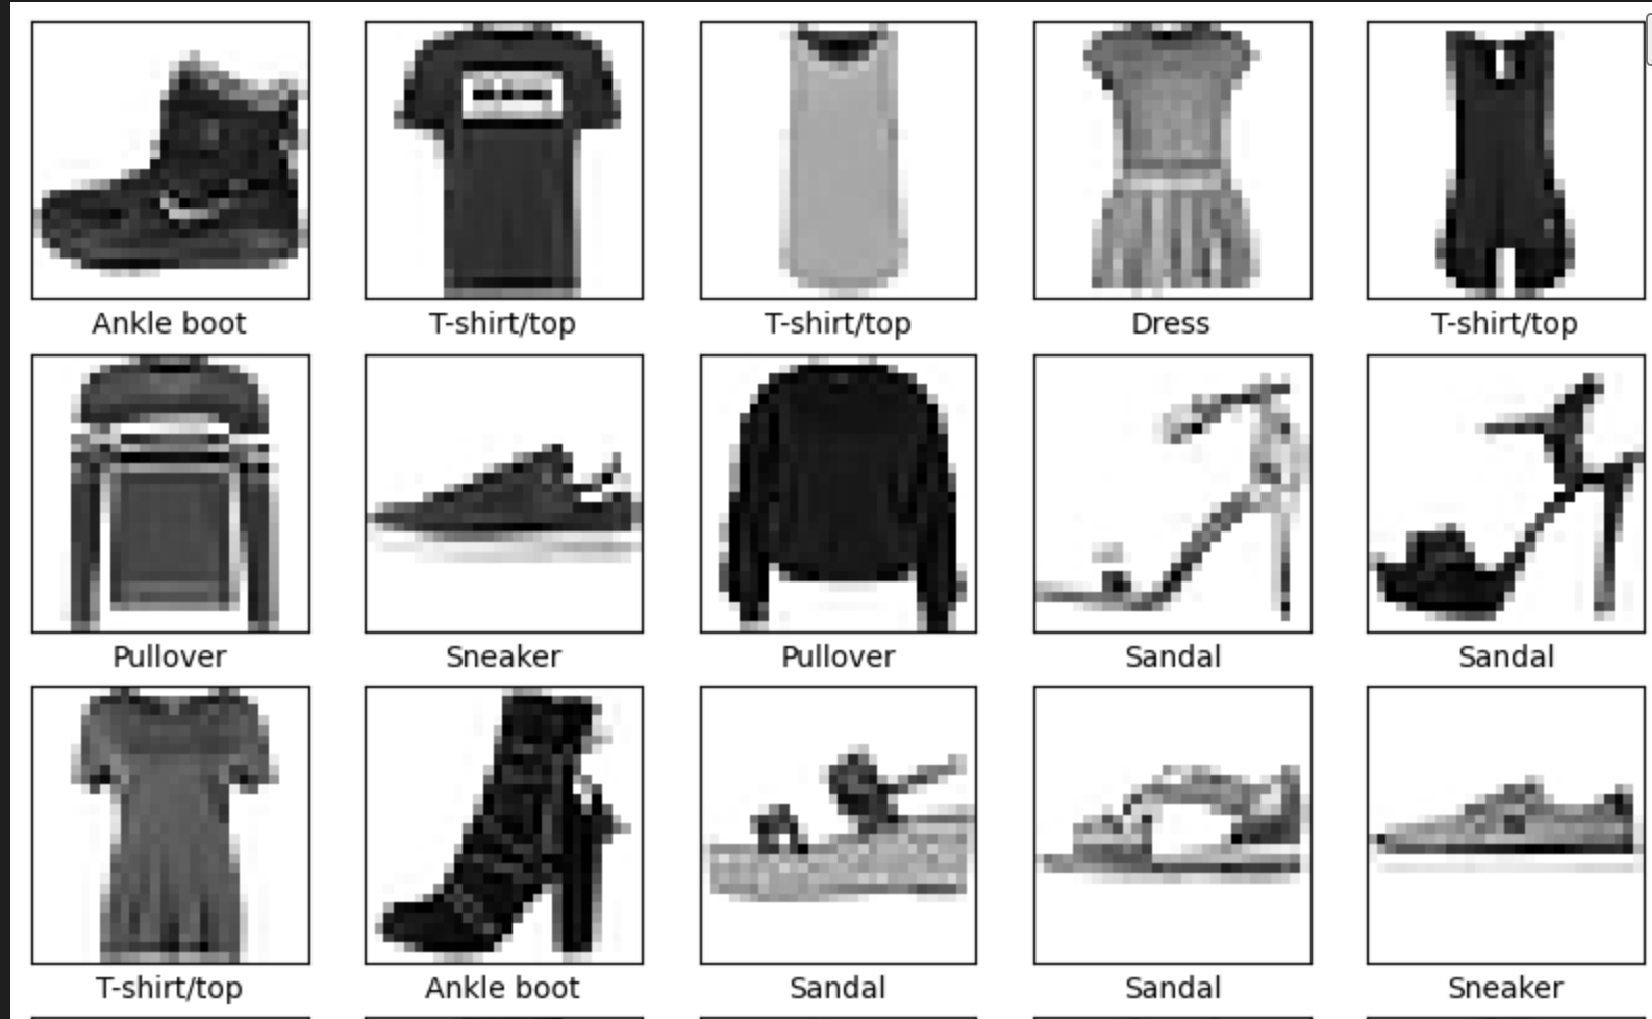
\includegraphics[width=8cm]{report/figures/example_items.pdf}
    \end{figure}
\end{frame}

\begin{frame}
    \myheading{Model build}
    \begin{enumerate}
        \item{Training set consisting of 60000 and and test set of 10000}
        \item First layer: 128 neruons and uses ReLu acivation function
        \item Second layer: 10 (one for each category) and uses soft max function to get the probabilities of each class
        \item Loss function: SparseCategoricalCrossEntropy
        \item One model for each optimizer, Adagrad, ADAM, SGD and RMSprop. 
    \end{enumerate}
\end{frame}

\end{document}